\chapter{Molecular Imaging Methods}
\label{sec:imaging}

This chapter introduces two molecular imaging methods, \textit{Computed Tomography} (CT) and 
\textit{Cryo-Electron Microscopy} (Cryo-EM). Their observation model is defined in a mathematical way and reconstruction is presented.
Finally, an abstraction is presented, as both methods are considered similar.




\section{Computed Tomography}
CT is a well established molecular imaging method.
Using X-ray sources, fan shaped beams are produced which scan the biological sample.
Through scanning over straight lines, many observations are collected, 
and the biological sample can be reconstructed\footnote{For additional information \cite{computedTomography}}.

\paragraph{2D Tomographic Observation:}

Mathematically, CT observations are defined as follows:

\begin{equation}
    \label{eq:2Dreconstruction}
    \begin{aligned}
        y_i[j] &= p_i + \eta_i[j] & \text{ with } 1 \leq i \leq N \text{ and } 1 \leq j \leq M \\
               &= R(x, \theta_i, s_j) + \eta_i[j] & \text{ with } 1 \leq i \leq N \text{ and } 1 \leq j \leq M
    \end{aligned}
\end{equation}

with
\begin{itemize}
    \item $x \in L^2(\Omega)$ : biological sample with $\Omega \subset \mathbb{R}^2 $ and $L^2$ Lebesgue space
    \item $R(\cdot; \theta_i, s_j): L^2(\Omega) \to \mathbb{R}^M , x \mapsto R(x; \theta_i, s_j)$ : Radon Transform\footnote{For additional information \cite{radonTransform}} 
        with $\theta_i \in SO(2)$ as observation angle and $s_j \in \mathbb{R}$ as sampling point
    \item $\eta_i \in \mathbb{R}^M$ : i.i.d Gaussian noise with $\eta_i[j] \sim \mathcal{N}(0,\sigma^2) \in \mathbb{R}$
\end{itemize}


\paragraph{Observation Illustration:}

The output of Radon Transform is called a \textit{sinogram}, which is a synonym for the CT observation.
In Figure~\ref{fig:phantom} the Shepp-Logan phantom is illustrated.
It is often used as an image for simulating a brain CT, and it refers to the biological sample $x$. 
Further, in Figure~\ref{fig:phantom_sinogram} and Figure~\ref{fig:phantom_sinogram_noisy} 
sinograms are presented with and without noise respectively. 
For this example, $\theta \in \mathbb{R}^{500}$ was evenly spaced
between $[0, 2 \pi]$ and $dim(s) = 400$. 
Thus, $p \in \mathbb{R}^{500 \times 400}$ and noise is added to reach an \snry of 10 dB.

\begin{figure}[H]
    \captionsetup[subfigure]{justification=centering}
    \centering
    \begin{subfigure}[t]{0.3\textwidth}
        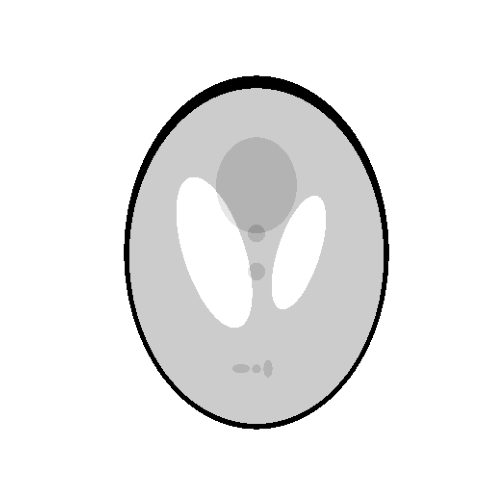
\includegraphics[width=\textwidth]{phantom.png}
        \caption{Shepp-Logan phantom: $x$}
        \label{fig:phantom}
    \end{subfigure}\hfill
    \begin{subfigure}[t]{0.3\textwidth}
      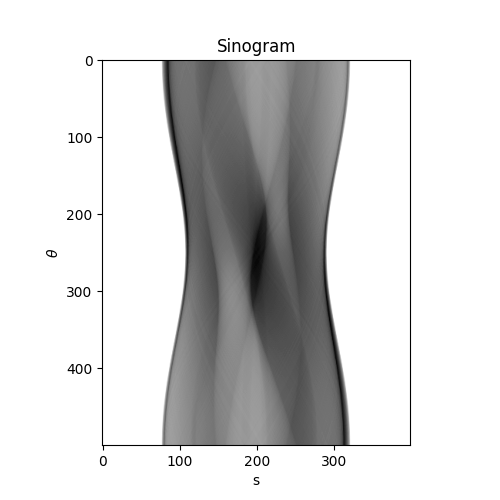
\includegraphics[width=\textwidth]{phantom_sino.png}
      \caption{Clean sinogram: $R(x, \theta, s)$}
      \label{fig:phantom_sinogram}
    \end{subfigure}\hfill
    \begin{subfigure}[t]{0.3\textwidth}
      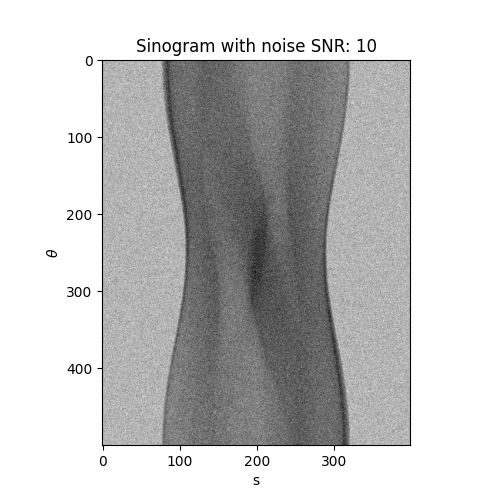
\includegraphics[width=\textwidth]{phantom_sino_noisy_snr10.png}
      \caption{Noisy sinogram: $R(x, \theta, s) + \eta = y + \eta$}
      \label{fig:phantom_sinogram_noisy}
    \end{subfigure}
    \caption{Shepp-Logan phantom and sinograms.}
    \label{fig:phantom_and_sinos}
  \end{figure}


\paragraph{Tomography Reconstruction:}

CT reconstruction is a popular Inverse Problem. 
The aim is to reconstruct a biological sample based on observations.
When the biological sample is in 2D, observations are available in 1D. 
The reconstruction is possible for 3D objects too, where observations are in 2D.
In this Thesis, I will focus on the 2D case of CT.


\subparagraph{Filter Backprojection:}
Filter Backprojection (FBP)~\cite{tomographicReconstruction} is a reconstruction method used in CT.
Until recently, it was the primary method for reconstruction as it allows to inverse the Radon Transform, resulting in 
$x^{\prime}$ which $ \approx x$ for the noiseless case. 

FBP can be defined as:

\begin{equation}
    \label{eq:fbp}
    \begin{aligned}
        \textit{FBP}(\cdot; \theta, s) : \mathbb{R}^{M \times N} \to\mathbb{R}^{M \times M}, y \mapsto \textit{FBP}(y; \theta, s) = x^{\prime}
    \end{aligned}
\end{equation}

Where $\theta$ are projection angles and $s$ are the sampling points.
But, the algorithm fails when working with highly noisy data~\cite{cryoEmMath2}, as it is not possible to draw meaningful
connections any longer, noise
is dominating information in the data.

Therefore, alternatives for the high noise domain have been studied in recent year.
Lately, neural network approaches emerged, which further processed the output of FBP to increase reconstruction quality.
This is the approach I will follow in this Thesis. \citet{ct-reconstruction-comparison} compared different 
Deep-Learning reconstruction methods for CT. 

\subparagraph{U-Net:}
Today's state-of-the-art reconstruction algorithms are Deep-Learning based.
U-Net~\cite{unet-tomography}, a convolution neural network, performed
much better compared to FBP in the comparison of \citet{ct-reconstruction-comparison}.
Therefore, it is an interesting baseline and additionally can be combined with other ideas.

In Figure~\ref{fig:phantom_fbps} reconstructions from Shepp-Logan phantom are presented.
\snry is defined to reach 10 dB.
The quality of the noisy reconstruction is rather low, some important details are missing, and noise dominates reconstruction.
If more noise is present in $y$, the reconstruction will be of even lower quality.
Further, Figure~\ref{fig:fbp_unet_phantom_noisy} 
shows reconstruction with U-Net where some details are missing as well, although overall noise is drastically decreased.


\begin{figure}[H]
    \captionsetup[subfigure]{justification=centering}
    \centering
    \begin{subfigure}[t]{0.3\textwidth}
        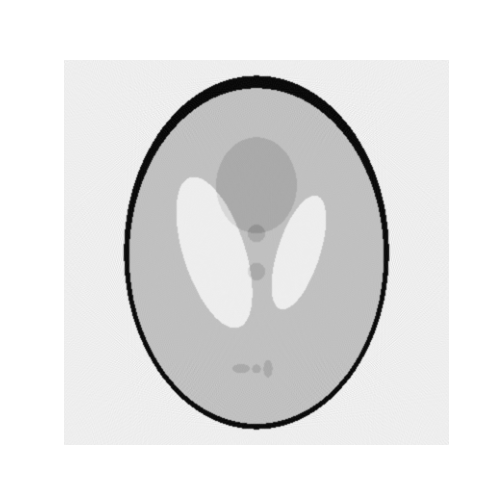
\includegraphics[width=\textwidth]{fbp_phantom_clean.png}
        \caption{Clean reconstruction: $\textit{FBP }(p, \theta, s)$}
        \label{fig:fbp_phantom}
    \end{subfigure}\hfill
    \begin{subfigure}[t]{0.3\textwidth}
      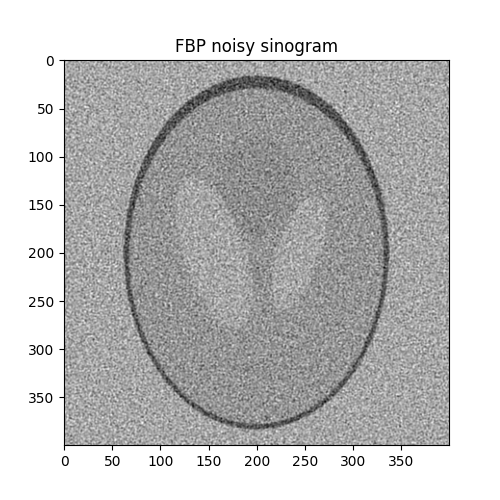
\includegraphics[width=\textwidth]{fbp_phantom_snr_10.png}
      \caption{Noisy reconstruction: $\textit{FBP }(y, \theta, s)$}
      \label{fig:fbp_phantom_noisy}
    \end{subfigure}\hfill
    \begin{subfigure}[t]{0.3\textwidth}
      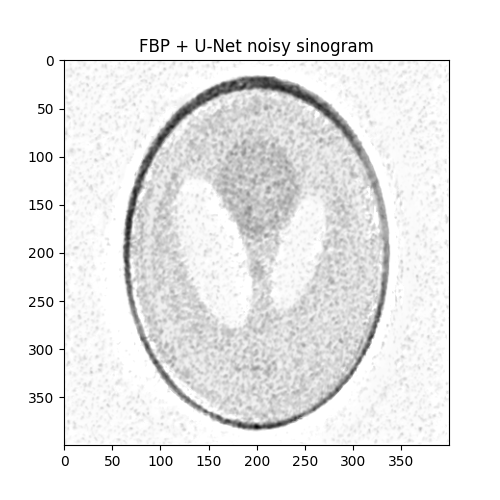
\includegraphics[width=\textwidth]{fbp_unet_phantom_snr_10.png}
      \caption{Noisy reconstruction: $\textit{UNet }(\textit{FBP }(y, \theta, s))$}
      \label{fig:fbp_unet_phantom_noisy}
    \end{subfigure}
    \caption{Shepp-Logan reconstructions with \snry 10 dB.}
    \label{fig:phantom_fbps}
  \end{figure}


\section{Cryo-Electron Microscopy}
Cryo-EM is another molecular imaging method, that enables the view of molecules in near-atomic resolution.
In this Thesis, for simplicity, only single-particle Cryo-EM~\cite{singleParticleCryoEm} is considered.
When writing about Cryo-EM it always refers to single-particle Cryo-EM.

During imaging, molecules are frozen in a thin layer of ice, where they are randomly oriented and positioned. 
Random orientation and positioning make reconstruction challenging, 
but freezing allows observation in a stable state where molecules are not moving.
2D tomographic projections of molecules are observed with an electron microscope, which are called \textit{micrograph}. 
Frozen molecules are fragile, and the electron microscope needs to work with
very low power (electron dose), resulting in highly noisy observations. The resulting SNR
is typically smaller than 0 dB~\cite{cryoEmMath2}.

In addition, observed molecules are not equal in the sense that there are some structural varieties between
molecules (isotopes). While observing the same molecule in ice many times, single observations could be from different isotopes.

\paragraph{3D Cryo-EM observation:}
Mathematically, observation is defined as follows:
\begin{equation}
    \label{eq:cryoEmSimple}
    \begin{aligned}
        y_i &= p_i + \eta_i &\text{ with } 1 \leq i \leq N,\\
        y_i &= \Pi_z  (\; Rot (\;x; \theta_i )) + \eta_i &\text{ with } 1 \leq i \leq N,    
    \end{aligned}
\end{equation}

where 
\begin{itemize}
    \item $x \in L^2(\Omega)$: biological sample with $\Omega \subset \mathbb{R}^3 $
    \item $\Pi_z : L^2(\Omega) \to L^2(\tilde{\Omega}), x \mapsto  \int x(\cdot,\cdot,z) dz$: z-axis projection operator
          with $\tilde{\Omega} \subset \mathbb{R}^2$
    \item $\theta_i = [\theta_i^{(1)}, \theta_i^{(2)}, \theta_i^{(3)} ] $: 3D rotation matrix with $ \theta_i^{(1)}, \theta_i^{(2)}, \theta_i^{(3)} \in [0, 2 \pi]$ and \\
          $R_{\theta_i} =  R_{e_x} (\theta_i^{(1)}) R_{e_y} (\theta_i^{(2)}) R_{e_z} (\theta_i^{(3)}) = [R^1_{\theta_i}, R^2_{\theta_i}, R^3_{\theta_i}] \in SO(3)$ 
          \footnote{For additional information see \ref{app:3DrotationMatrix}}
          
    \item $\textit{Rot} : L^2(\Omega) \to L^2(\Omega), \textit{Rot}(x, \theta_i) = \left((x_1,x_2,x_3) \mapsto ( x_1R^1_{\theta_i}, x_2R^2_{\theta_i}, x_3R^3_{\theta_i})\right)$: rotation operator
    \item $\eta_i \in \mathbb{R}^M$: i.i.d Gaussian noise with $\eta_i[j] \sim \mathcal{N}(0,\sigma^2) \in \mathbb{R}$
\end{itemize}

% $y_i \in \mathbb{R}^M$ with $M$ as observation dimension.

% Then, $\Pi_z : L^2(\Omega) \to L^2(\tilde{\Omega}), x \mapsto  \int x(\cdot,\cdot,z) dz$ is projection operator from z-axis
% and $Rot : L^2(\Omega) \to L^2(\Omega), Rot(x, \theta_i) = \left((x_1,x_2,x_3) \mapsto x( x_1R^1_{\theta_i}, x_2R^2_{\theta_i}, x_3R^3_{\theta_i})\right)$ is rotation operator modelling the rotation during freezing.
% Further, $\theta_i = [\theta_i^{(1)}, \theta_i^{(2)}, \theta_i^{(3)} ] $ where entries $ \theta_i^{(1)}, \theta_i^{(2)}, \theta_i^{(3)} \in \mathbb{R}$ and 
% $R_{\theta_i} =  R_{e_x} (\theta_i^{(1)}) R_{e_y} (\theta_i^{(2)}) R_{e_z} (\theta_i^{(3)}) = [R^1_{\theta_i}, R^2_{\theta_i}, R^3_{\theta_i}] \in SO(3)$ is the 3D rotation matrix 
% (see \ref{app:3DrotationMatrix} for further details). 
% $\eta_i \sim \mathcal{N}(0,\sigma^2I) \in \mathbb{R}^M$ corresponds to noise of observation.

Equation~\ref{eq:cryoEmSimple} is a simplified version of Cryo-EM.
First, the point spread function of the microscope is not taken into account.
Second, structural variety is ignored, the underlying sample $x$ is not the same 
for every observation. 
Precisely, $x$ can be seen as a random signal from an unknown distribution defined over all possible molecule structures.
In this Thesis, only the simplified version is considered.

Moreover, as $y_i$ is not observable directly, discretization is needed:
\begin{equation}
    \label{eq:cryoEmSimpleDiscrete}
    \begin{aligned}
        y_i &= \left( \Pi_z (\; Rot (\;x; \theta_i)) + \eta_i\right)(\Delta) & \text{ with } 1 \leq i \leq N \\
        y_i[j,k] &= \Pi_z (\; Rot(\;x; \theta_i))_{j,k} + \eta_i[j,k] & \text{ with } 1 \leq i \leq N \text{ and } 1 \leq j,k \leq \sqrt{M}
    \end{aligned}
\end{equation}

With
\begin{itemize}
    \item $\Delta \in \tilde{\Omega}^{M}$: sampling grid with dimension $M$
    \item $y_i[j,k]$, $\eta_i[j,k]$ and $\Pi_z(\cdot)_{j,k}$ $ \in \mathbb{R}$ with $j,k$ as indices of the sampling grid.
\end{itemize}
% $\Delta \subset \tilde{\Omega}^{M^2}$ is the sampling grid with dimension $M^2$.
% Further, $y[j,k]$, $\eta[j,k]$ and $\Pi_z(\cdot)_{j,k}$ $ \in \mathbb{R}$ with $j,k$ as indices of 
% the sampling grid.


\paragraph{Observation Illustration:}
In Figure~\ref{fig:cryo-em-omicron} Cryo-EM micrographs are illustrated as well as the reconstructed biological sample.

\begin{figure}[H]
    \captionsetup[subfigure]{justification=centering}
    \centering
    \begin{subfigure}[t]{0.2\textwidth}
        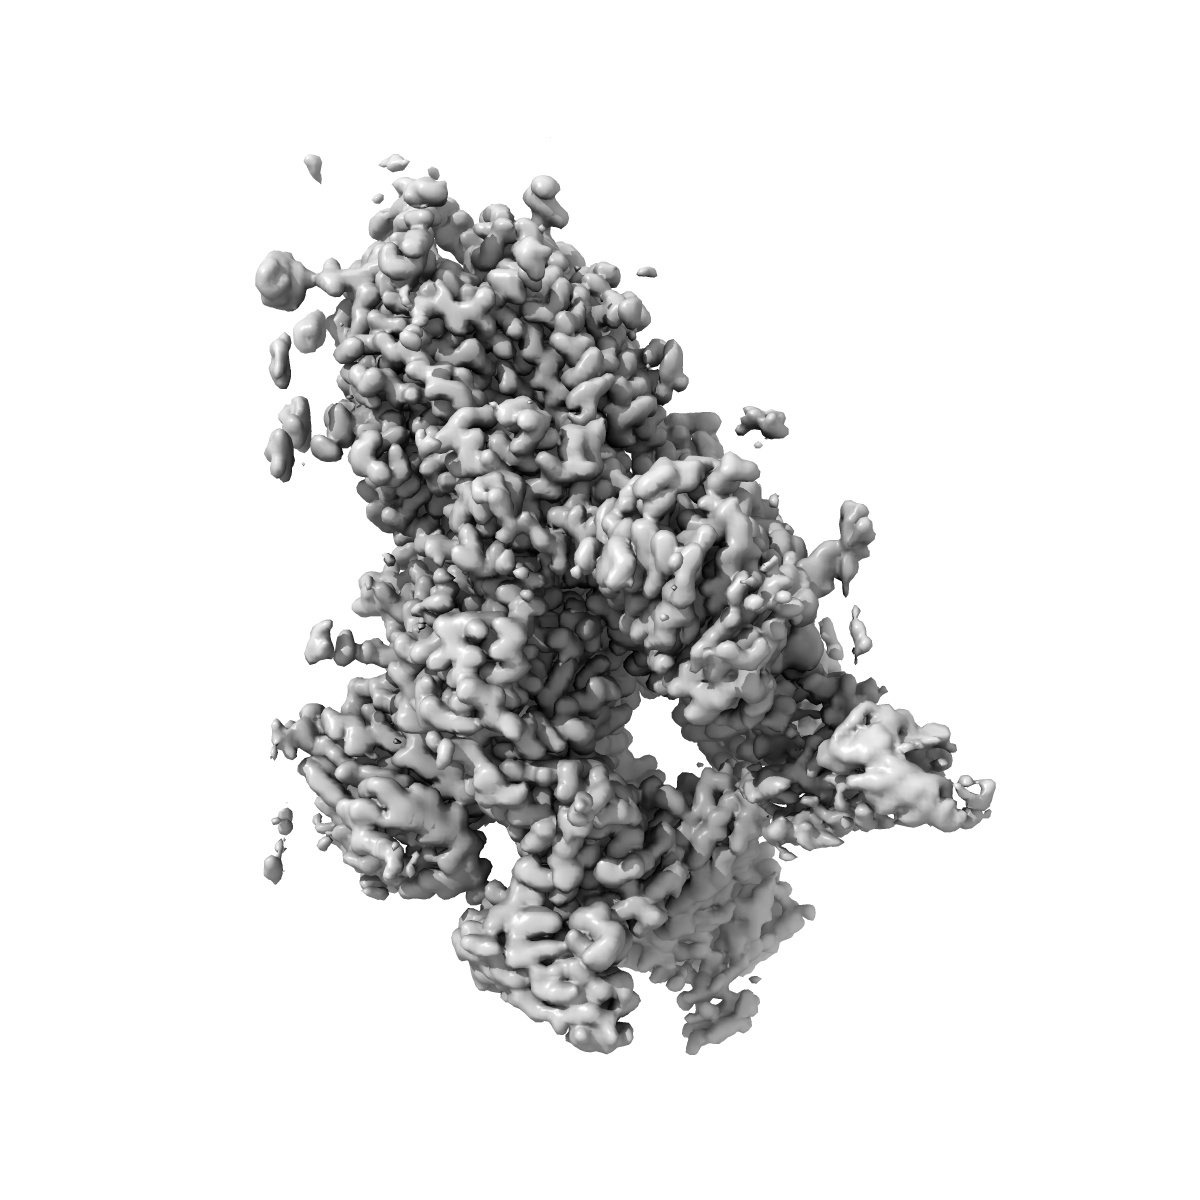
\includegraphics[width=\textwidth]{emd_32500.map_xsurface.jpeg}
        \caption{COVID-19 Omicron spike: $x^{\prime}$}
    \end{subfigure} \hfill
    \begin{subfigure}[t]{0.2\textwidth}
      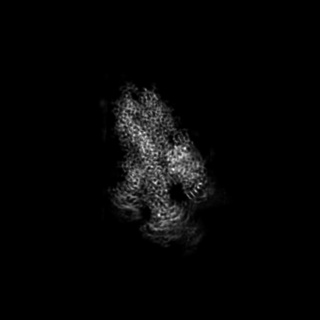
\includegraphics[width=\textwidth]{emd_32500.map_xprojection.jpeg}
      \caption{Micrograph along x-axis}
    \end{subfigure}\hfill
    \begin{subfigure}[t]{0.2\textwidth}
      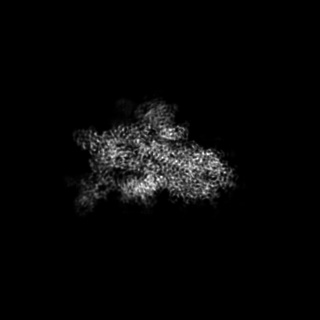
\includegraphics[width=\textwidth]{emd_32500.map_yprojection.jpeg}
      \caption{Micrograph along y-axis}
    \end{subfigure}\hfill
    \begin{subfigure}[t]{0.2\textwidth}
        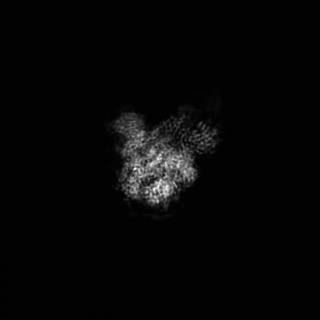
\includegraphics[width=\textwidth]{emd_32500.map_zprojection.jpeg}
        \caption{Micrograph along z-axis}
      \end{subfigure}
    \caption{Cryo-EM reconstruction and micrographs of COVID-19 Omicron spike\protect\footnotemark.}
    \label{fig:cryo-em-omicron}
  \end{figure}

\footnotetext{\url{https://www.ebi.ac.uk/emdb/EMD-32500}}

\paragraph{Cryo-EM Reconstruction:}
Cryo-EM reconstruction is defined as the approximation of a 3D object from 2D observations.
Cryo-EM reconstruction is computationally intensive and multiple steps are required to get from 
observations to the final structure\footnote{For additional information \cite{singleParticleCryoEm, cryoEmMath}}.


\section{Abstraction}
As CT and Cryo-EM are highly related, the aim of this section is to define
an abstraction model. The big difference is, that CT is in 2D and Cryo-EM in 3D.
Mathematically, an extension from 2D to 3D should be theoretically feasible. 
It is considered a numerical challenge due to the need of additional computing resources.
Therefore, an abstract form will be defined.
A similar notation than previously is used, with the biological sample $x \in L^2(\Omega)$.
Further, the biological sample dimension space is parametrized with $D$, consequently $\Omega \subset \mathbb{R}^D$.
Additionally, dimension of observation space is defined as $D-1$, such that 
$\tilde{\Omega} \subset \mathbb{R}^{D-1}$.


\begin{equation}
    \label{eq:abstract-model}
    \begin{aligned}
        y_i &= p_i + \eta_i (\Delta) & \text{ with } 1 \leq i \leq N \\
        y_i &= \left( A(x, \theta_i) + \eta_i \right) (\Delta) & \text{ with } 1 \leq i \leq N 
    \end{aligned}
\end{equation}
with
\begin{itemize}
    \item $x \in L^2(\Omega)$: biological sample
    \item $A: L^2(\Omega) \to \mathbb{R}^M, x \mapsto A(x; \theta_i)$: a non-linear operator 
    \item $\theta_i \in SO(D)$: projection angle(s) vector, with $P$ projection dimension
    \item $\eta_i \in \mathbb{R}^M$: i.i.d Gaussian noise with $\eta_i[j] \sim \mathcal{N}(0,\sigma^2) \in \mathbb{R}$
    \item $\Delta \in \tilde{\Omega}^{M}$: term for discretization
\end{itemize}

\paragraph{Reconstruction:}

Further, an abstract form of the reconstruction operator is defined as:

\begin{equation}
    \textit{Recon} : \mathbb{R}^{M \times N} \to \mathbb{R}^{M \times M}, y \mapsto Recon(y; \theta)
\end{equation}

With $\theta_i \in SO(D)$ as the projection angle(s).

For CT, parameter $D=2$ and $A(\cdot)$ is the Radon Transform.
Further, reconstruction operator can be defined as FBP (with or without U-Net).
Cryo-EM parameters are defined with $D=3$ and $A(\cdot)$ can be
defined as $\Pi_z \left(\; \textit{Rot}(\;x; \theta) \right)$. 


\paragraph{High Noise Regime:}
Cryo-EM observations are highly noisy, which makes reconstruction challenging. 
There are different ways to reduce noise from observations, most of them are related to averaging. 
Averaging needs to consider similar observations and ignore diverse ones. 
In the defined abstract model, averaging over paired observations from $\theta$ should be a good averaging model.

One idea would be to measure distances between observations.
Another way is to find a low-dimensional embedding which maps observation $y$ to $\theta$.
When talking from low-dimensional embeddings, there is no way around Graph Laplacian and Graph Learning,
which will be introduced in the next chapter.
